\documentclass{article}

% Português
\usepackage[brazilian]{babel}
% Define margens
\usepackage[a4paper,margin=1in]{geometry}
% Tabelas bonitas
\usepackage{booktabs,multirow}
% Símbolos matemáticos
\usepackage{amsmath}
\usepackage{amssymb}
\usepackage{gensymb}
% Figuras
\usepackage{graphicx}
% Legendas em subfiguras
\usepackage{subcaption}
% Mostar tabelas grandes em páginas no modo paisagem
\usepackage{pdflscape}
\usepackage{afterpage}


\title{COS868 - Projeto do curso}
\author{Fernando Dias}
\date{5 de Janeiro de 2025}

\begin{document}

\maketitle

Este é o relatório do projeto do curso de probabilidade e estatística do Programa de Engenharia em Sistemas de Computação (PESC) da COPPE/UFRJ. Esse curso foi ministrado no trimestre 2024/3 pela professora Rosa Leão.

O código utilizado para a obtenção dos gráficos e tabelas está disponível em https://github.com/Fdms-3741/trabalhoprobabilidade.

\section{Introdução}

O objetivo desse trabalho é fazer uma avaliação estatística das taxas de download e upload de dois tipos de dispositivos: Smart TVs e Chromecasts. Nessa análise, investiga-se a distribuição das taxas enviadas e recebidas de modo a avaliar se essas distribuições seguem alguma distribuição conhecida da literatura. Além disso, é feito um teste comparativo entre as diferentes taxas para verificar se ambas seguem uma mesma distribuição.

Para esse trabalho, utilizou-se a linguagem \texttt{Python3} para construção de scripts que processam os datasets e geram as tabelas e gráficos deste relatório. As bibliotecas \texttt{numpy} e \texttt{scipy} são utilizadas para operações numéricas em arrays e calcular algumas das estatísticas vistas nesse relatório. A biblioteca \texttt{pandas} é responsável por manipular o dataset através de tabelas. As bibliotecas \texttt{matplotlib}, \texttt{seaborn} e \texttt{statsmodels} foram utilizadas para criar os gráficos.

A metodologia para cálculo dos dados é a mesma para todas as questões: Primeiramente, ambos os arquivos CSV são importados e unidos em um único dataset. Após isso, o dataset é transformado em um \texttt{pandas.DataFrame} que contém as colunas descritas na tabela~\ref{tab:colunas_dataset}. Com o dataset nesse formato, os gráficos, tabelas e boxplots são gerados diretamente através da biblioteca \texttt{seaborn}, que automaticamente filtra e separa os dados dessa tabela para a criação de multiplos gráficos.

\begin{table}[h]
	\centering
	\begin{tabular}{rll}
		\toprule
		Nome                & Tipo                    & Descrição                                        \\
		\midrule
		Data e hora         & \texttt{datetime[64]ns} & Data e hora da observação                        \\
		Tipo de dispositivo & Smart TV|Chromecast     & Separa dispositivos entre Chromecast ou Smart TV \\
		Direção do fluxo    & Upload|Download         & Define se o bps é de upload ou de download       \\
		bps                 & \texttt{float}          & Valor de bps naquele minuto                      \\
	\end{tabular}
	\caption{Colunas dos datasets gerais}
	\label{tab:colunas_dataset}
\end{table}


\subsection{Tratamento dos valores nulos}

Os valores de taxas consistem em valores que variam em diversas ordens de grandeza. Portanto, é necessário um tratamento dos dados para que as estatísticas possam ser calculadas sem o risco de perda de precisão. A sugestão dada pelo roteiro do projeto consiste em calcular a estatística do $\log$ dos dados ao invés dos próprios valores. Isso porém

A primeira alternativa para lidar com o problema da existencia de zeros nos dados consiste em calcular o logaritmo dos valores somados a 1. Assim, todas as entradas nulas serão consideradas e terão valor 0 e o erro para entradas grandes é negligenciável. Uma segunda consequência é o limitar o conjunto de dados na região $[0,\infty)$, que impede que valores bem pequenos de bps se tornem outliers com ordem de grandeza muito grande. A operação de conversão seguiu a seguinte fórmula:
\begin{equation*}
	b'_n = \log_{10}(b_n+1)\;\forall\;n
\end{equation*}

A segunda alternativa consiste em tirar os valores 0 das entradas antes de fazer o logaritmo. Para manter consistência entre datasets e preservar a região do conjunto de dados, a mesma função de conversão é utilizada em ambos os casos.

A escolha entre os datasets vai depender da interpretação desejada dos resultados obtidos e dos objetivos com a análise, já que ambos os datasets fornecem resultados diferentes. Ao longo desse trabalho, é possível ver situações onde um dataset é mais apropriado para explicar um fenômeno do que outro, e essas situações serão elencadas ao longo desse trabalho.

\section{Estatísticas gerais}
\label{sec:estatistica-geral}

Para as estatísticas gerais, os dados foram divididos em quatro conjuntos distintos: Upload e download da Smart TV e upload e download do Chromecast. Os resultados para as estatísticas gerais podem ser vistas na tabela~\ref{tab:questao2-estatisticas-globais}. Já os histogramas, com e sem exclusão de zeros, e as CDFs empíricas podem ser vistas nas figuras~\ref{fig:questao2-histogramas-com-zeros},~\ref{fig:questao2-histogramas-sem-zeros} e~\ref{fig:questao2-ecdf} respectivamente. Os boxplots representando os dois datasets está na figura~\ref{fig:questao2-boxplots}.

\begin{table}[h]
	\centering
	\begin{tabular}{llrrrr}
\toprule
 &  & count & average & std_dev & variance \\
device_type & flow_type &  &  &  &  \\
\midrule
\multirow[t]{2}{*}{Chromecast} & bytes_down & 1620529 & 3.800046 & 1.663896 & 1.289921 \\
 & bytes_up & 1620529 & 3.350300 & 0.459969 & 0.678210 \\
\cline{1-6}
\multirow[t]{2}{*}{Smart TV} & bytes_down & 4417903 & 2.351679 & 6.721324 & 2.592552 \\
 & bytes_up & 4417903 & 2.158288 & 4.110139 & 2.027348 \\
\cline{1-6}
\bottomrule
\end{tabular}

	\caption{Estatísticas globais}
	\label{tab:questao2-estatisticas-globais}
\end{table}


Na tabela~\ref{tab:questao2-estatisticas-globais}, vemos as estatísticas globais de cada conjunto de dados analisado, além da quantidade de entradas em cada. Vemos que, para cada tipo de dispositivo, as médias das taxas são próximas, porém o download possui um desvio padrão significativamente maior que o upload. Isso indica que alguma característica do download torna a taxa mais variável do que a taxa do upload, o que pode ser explicado pelos diferentes tipos de taxas para diferentes serviços de streaming. Já o desvio padrão é da mesma ordem de grandeza, e as vezes até maior, do que a média em todos os casos. Isso é um indício de um grande espalhamento dos dados, o que pode ser esperado de dispositivos que podem alternar entre períodos de alta demanda (streaming de vídeo em 4K) ou baixa demanda (música ou desligado).

\begin{figure}[h]
	\centering
	\caption{Histogramas dos dados com a \textbf{inclusão} de valores nulos}
	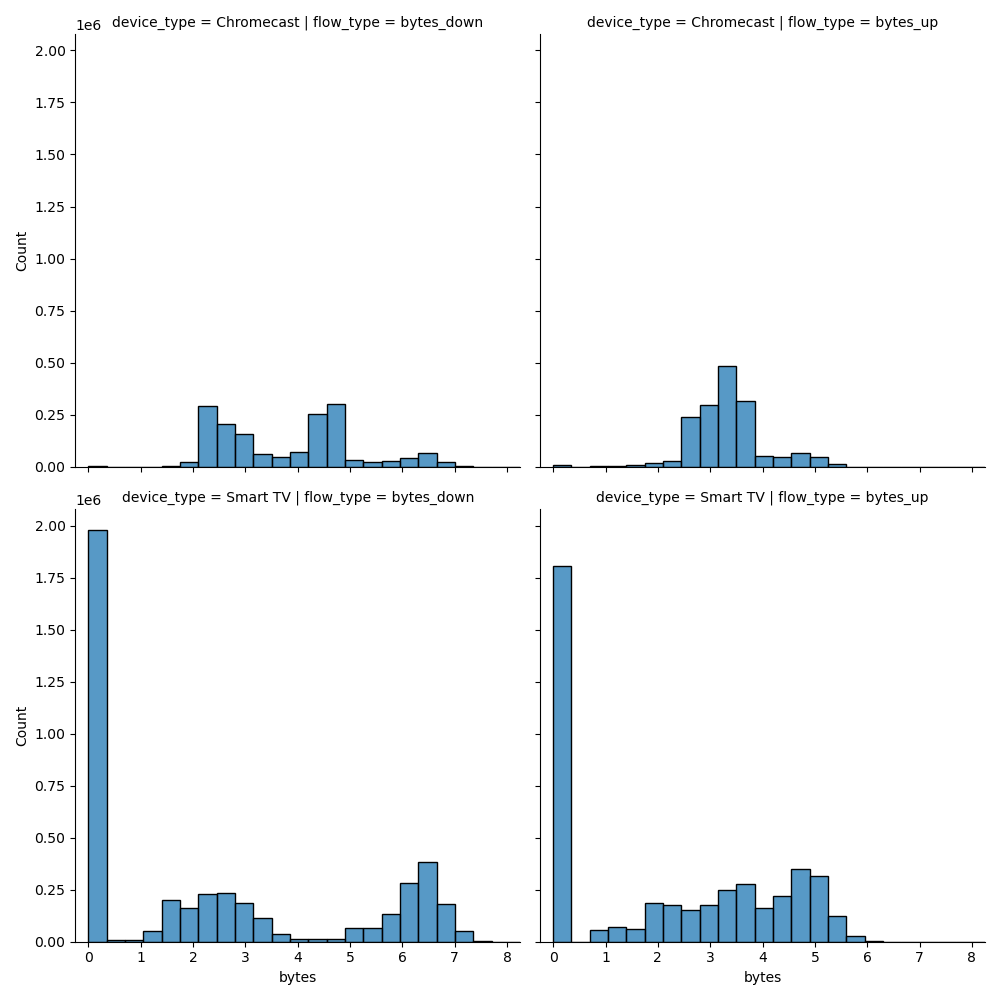
\includegraphics[width=\textwidth]{./resultados/questao2/histograms_add1.png}
	\label{fig:questao2-histogramas-com-zeros}
\end{figure}

Vemos os datasets sendo representados integralmente pelos histogramas da figura~\ref{fig:questao2-histogramas-com-zeros}. Em todos os histogramas \textit{do relatório}, os bins dos histogramas foram calculados utilizando a regra de sturges onde $bins=\lceil1+\log_2(n)\rceil$. Uma primeira diferença notável está no impacto que a presença de zeros tem no formato do histograma dos conjuntos de dados das Smart TVs. Esse comportamento não foi observado no Chromecast e, sem mais detalhes sobre como o experimento foi conduzido, não é possível apontar o motivo dessa diferença.

\begin{figure}[h]
	\centering
	\caption{Histogramas dos dados com a \textbf{exclusão} de valores nulos}
	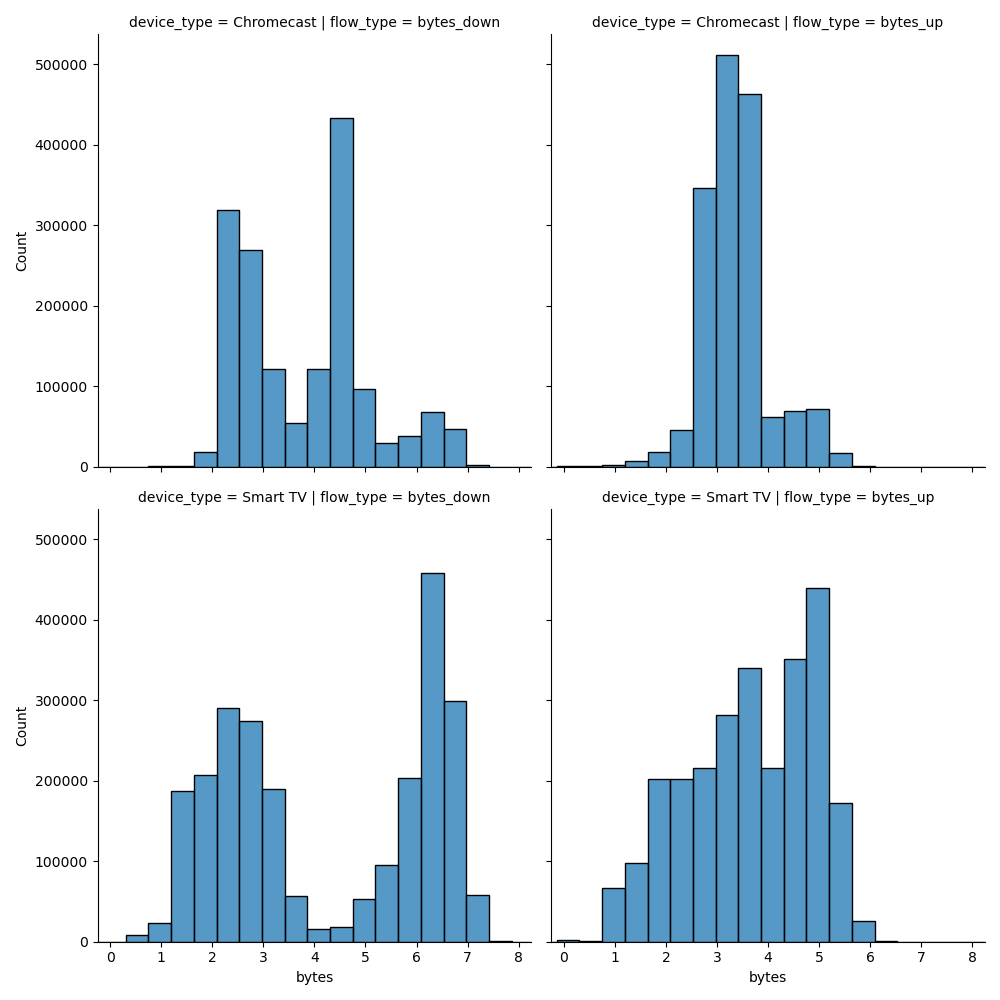
\includegraphics[width=\textwidth]{./resultados/questao2/histograms_dropna.png}
	\label{fig:questao2-histogramas-sem-zeros}
\end{figure}

Com a remoção dos valores nulos, é possível observar com mais detalhes o formato do histogramas na figura~\ref{fig:questao2-histogramas-sem-zeros}. Nessa figura, podemos distinguir a presença de uma distribuição multimodal nos histogramas de download comparado aos histogramas de upload. Isso pode ser explicado devido a presença de variáveis independentes que afetam o padrão de transmissão de dados, mas sem mais informações sobre os dispositivos não é possível definir a causa desse comportamento. As distribuições de upload não parecem possuir esse comportamento multimodal, e a distribuição da Smart TV possui um espalhamento maior do que a distribuição do :/Chromecast.



\begin{figure}[h]
	\centering
	\caption{CDFs empíricas dos dados com a inclusão de valores nulos}
	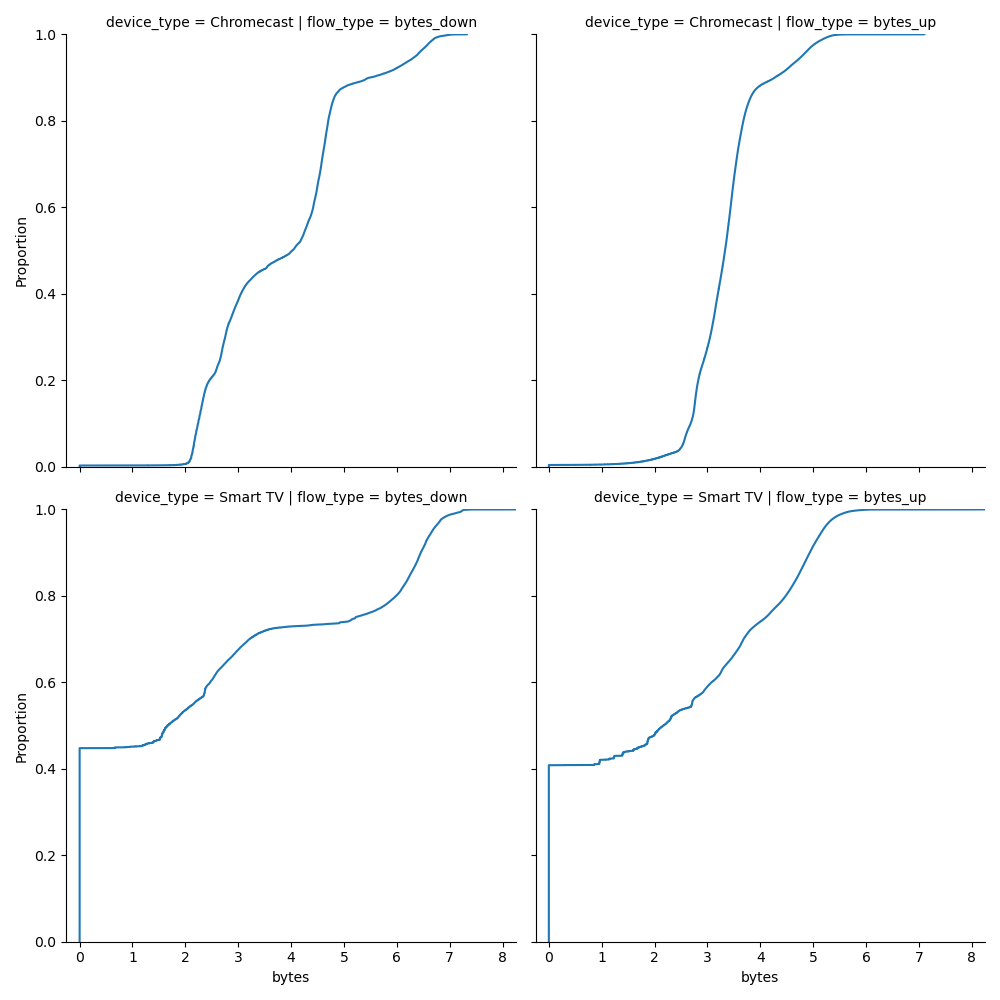
\includegraphics[width=\textwidth]{./resultados/questao2/ecdfs_add1.png}
	\label{fig:questao2-ecdf}
\end{figure}

Através da distribuição cumulativa empírica da figura~\ref{fig:questao2-ecdf}, podemos fazer as mesmas observações feitas através do histograma, o que mostra que a escolha dos bins foi bem representativa. As observações sobre o comportamento multimodal e o espalhamento do dataset são feitos através da observação da variação da taxa de crescimento da curva. Para observar o efeito multimodal nos gráficos de download, é possível observar que há duas partes do gráfico onde o crescimento da curva aparenta ``acelerar'' com mais rapidez do que as demais regiões. Já para o espalhamento, é possível observar que o crescimento da curva se encontra sobre uma região do eixo X menor no caso do Chromecast do que no caso da Smart TV, o que indica uma maior concentração de dados em uma região de suporte menor, ou seja, um menor espalhamento dos dados.

\begin{figure}[h]
	\centering
	\begin{subfigure}{0.47\textwidth}
		\centering
		\caption{Sem exclusão de zeros}
		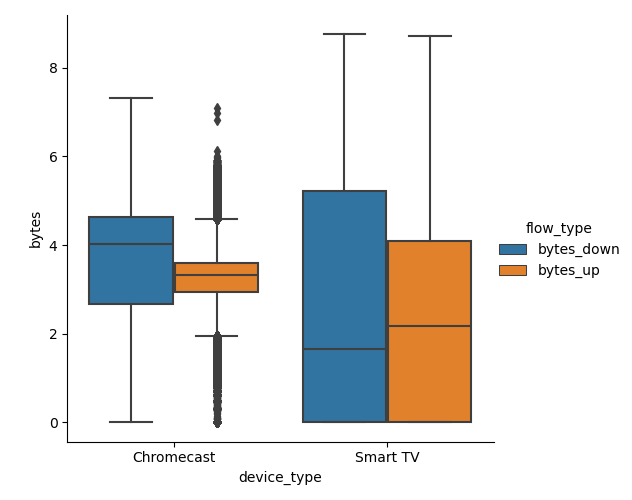
\includegraphics[width=\textwidth]{./resultados/questao2/boxplots_add1.png}
		\label{fig:questao2-boxplots-sem-exclusao}
	\end{subfigure}
	\hfill
	\begin{subfigure}{0.47\textwidth}
		\centering
		\caption{Com exclusão de zeros}
		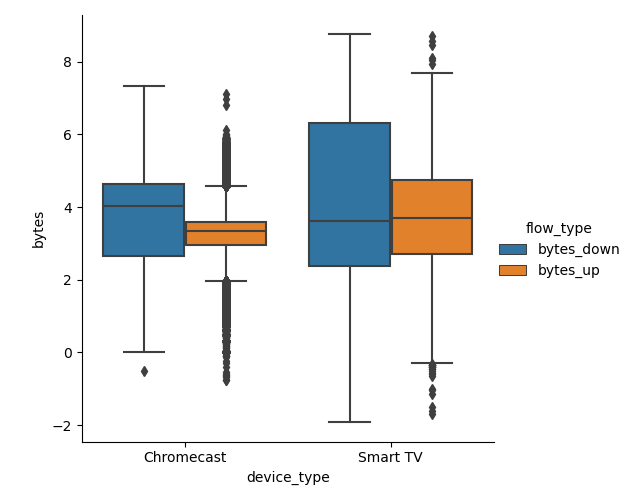
\includegraphics[width=\textwidth]{./resultados/questao2/boxplots_dropna.png}
		\label{fig:questao2-boxplots-com-exclusao}
	\end{subfigure}
	\caption{Boxplot dos dados gerais}
	\label{fig:questao2-boxplots}
\end{figure}

Os boxplots da figura~\ref{fig:questao2-boxplots} servem tanto para fazer uma comparação direta entre os quatro datasets quanto para observar o efeito da exclusão dos valores nulos. Na figura~\ref{fig:questao2-boxplots-com-exclusao} o efeito dos valores nulos só está presente nos dados da Smart TV, como observado anteriormente nos histogramas, e o efeito disso é o maior tamanho da distância inter-quartis (IQR) do que nos dados do chromecast. Ademais, como o fundo do box está em 0 em ambos os casos, sabemos que ao menos 25\% dos dados nesses datasets é de valores nulos.

Com a exclusão dos zeros, como visto na figura~\ref{fig:questao2-boxplots-sem-exclusao}, os dados de um dispositivo já apresentam um comportamento similar aos dados do segundo dispositivo. Pode-se observar que os boxes da smarttv possuem uma distância interquartil maior que os boxes do Chromecast, tanto no caso de download quanto do upload. Vemos que o efeito do espalhamento afeta o formato dos whiskers e a aparição de outliers entre os dados de download e upload de ambos os dispositivos, mas a informação de multimodalidade não é observável. Com esse gráfico, podemos comparar apenas as estatísticas gerais entre os datasets de uma forma mais visual do que a observação em tabelas, porém nem todas as características do dataset puderam ser exploradas. Uma alternativa para observar a multimodalidade nesse tipo de visualização é utilizar um gráfico do tipo \texttt{violinplot}.

Nessa seção, as observações mais relevantes são elencadas a seguir:
\begin{itemize}
	\item A exclusão dos valores nulos tem um impacto significativo na distribuição da Smart TV
	\item Todos os dados possuem uma variância bem alta
	\item A distribuição para o Download possui dois picos característicos de uma multimodal, enquanto o upload não apresenta essa característica.
	\item Visualmente, é possível ver que a Smart TV apresenta distribuições que são mais espalhadas do que o Chromecast.
	\item As diferenças observadas podem ser resultado de diferentes tipos de serviços em um tipo de dispositivo que exigem taxas diferentes de consumo do que no outro, porém não é possível definir se esse é o caso sem mais informações sobre o experimento.
\end{itemize}

\section{Estatísticas por horário}
\label{sec:estatistica-horario}

Nessa análise, será feita a observação de estatísticas gerais por horário. O objetivo é observar diferenças no padrão de distribuição de dados devido a hora de observação. Para isso cada um dos quatro datasets observados anteriormente são divididos em 24 subconjuntos de dados, um para cada hora do dia, onde todos os dias e todos os dispositivos de cada conjunto são utilizados para a formação dos dados. A tabela~\ref{tab:questao3-estatisticas-horario} contém todas as estatísticas separadas por horário, e os gráficos das figuras~\ref{fig:questao3-variacao-media},~\ref{fig:questao3-variacao-std} e~\ref{fig:questao3-variacao-var} mostram as variações da média, desvio padrão e variância nos quatro datasets por horário, respectivamente. Finalmente, a figura~\ref{fig:questao3-boxplots} mostra os boxplots dos quatro conjuntos de dados, com cada box referente a uma hora do dia.

Um dos objetivos dessa análise é encontrar qual o horário de pico, ou seja, o horário com o maior tráfego médio observado entre os quatro datasets. Para encontrar esse dado, é necessário contabilizar o tráfego de todos os dispositivos observados, mesmo que o dispositivo não esteja transmitindo nem recebendo dados. Assim, será utilizado nessa análise os dados sem a exclusão das entradas nulas. Para comparar os efeitos da exclusão dos zeros, temos a tabela~\ref{tab:questao3-comparacao-zeros}. Vemos que, com a exclusão dos zeros, a diferença entre a menor média e a maior média é de no máximo 0.9 $\log(\text{bps})$, com todos os resultados entre 3 e 4.5. Já com o acréscimo dos zeros, os resultados de média variam significativamente (entre 0.7 e 3.4) para o caso da Smart TV, o que mostra que a disparidade entre os resultados observados dos dois dispositivos se dá pela adição dos zeros.

\begin{table}[h]
	\centering
	\begin{tabular}{llrrrr}
\toprule
 &  & \multicolumn{2}{r}{Sem zeros} & \multicolumn{2}{r}{Com zeros} \\
 &  & Mínimo & Máximo & Mínimo & Máximo \\
Tipo de dispositivo & Direção do fluxo &  &  &  &  \\
\midrule
\multirow[t]{2}{*}{Chromecast} & Download & 3.572052 & 4.077841 & 3.565706 & 4.052698 \\
 & Upload & 3.161117 & 3.542044 & 3.156929 & 3.521546 \\
\cline{1-6}
\multirow[t]{2}{*}{Smart TV} & Download & 3.697172 & 4.519928 & 0.735541 & 3.396095 \\
 & Upload & 2.938141 & 3.831448 & 0.768513 & 3.124258 \\
\cline{1-6}
\bottomrule
\end{tabular}

	\caption{Comparação da média com a exclusão dos zeros}
	\label{tab:questao3-comparacao-zeros}
\end{table}

\afterpage{
	\clearpage
	\thispagestyle{empty}
	\begin{landscape}
		\centering
		\begin{table}[h]
			\small
			\begin{tabular}{lrrrrrrrrrrrr}
	\toprule
	Tipo de dispositivo & \multicolumn{6}{r}{Chromecast} & \multicolumn{6}{r}{Smart TV}                                                                                                                                                         \\
	Direção do fluxo    & \multicolumn{3}{r}{Download}   & \multicolumn{3}{r}{Upload}   & \multicolumn{3}{r}{Download} & \multicolumn{3}{r}{Upload}                                                                                             \\
	                    & Desvio padrão                  & Média                        & Variância                    & Desvio padrão              & Média & Variância & Desvio padrão & Média & Variância & Desvio padrão & Média & Variância \\
	Hora                &                                &                              &                              &                            &       &           &               &       &           &               &       &           \\
	\midrule
	0                   & 1.408                          & 3.976                        & 1.983                        & 0.731                      & 3.461 & 0.534     & 1.976         & 4.511 & 3.905     & 1.242         & 3.667 & 1.544     \\
	1                   & 1.301                          & 3.790                        & 1.693                        & 0.653                      & 3.339 & 0.427     & 1.971         & 4.519 & 3.888     & 1.282         & 3.567 & 1.644     \\
	2                   & 1.201                          & 3.689                        & 1.444                        & 0.569                      & 3.248 & 0.324     & 1.989         & 4.353 & 3.959     & 1.311         & 3.376 & 1.720     \\
	3                   & 1.183                          & 3.638                        & 1.401                        & 0.548                      & 3.204 & 0.300     & 1.951         & 3.984 & 3.806     & 1.287         & 3.121 & 1.657     \\
	4                   & 1.185                          & 3.620                        & 1.406                        & 0.550                      & 3.181 & 0.303     & 1.887         & 3.697 & 3.562     & 1.218         & 2.938 & 1.484     \\
	5                   & 1.171                          & 3.572                        & 1.372                        & 0.533                      & 3.161 & 0.284     & 1.926         & 3.888 & 3.711     & 1.217         & 3.072 & 1.481     \\
	6                   & 1.162                          & 3.572                        & 1.350                        & 0.528                      & 3.164 & 0.279     & 1.924         & 3.835 & 3.704     & 1.209         & 3.134 & 1.461     \\
	7                   & 1.185                          & 3.622                        & 1.406                        & 0.559                      & 3.208 & 0.313     & 1.956         & 3.762 & 3.827     & 1.259         & 3.208 & 1.586     \\
	8                   & 1.204                          & 3.663                        & 1.451                        & 0.591                      & 3.254 & 0.349     & 2.052         & 4.036 & 4.214     & 1.328         & 3.409 & 1.765     \\
	9                   & 1.218                          & 3.704                        & 1.483                        & 0.605                      & 3.295 & 0.366     & 2.053         & 4.214 & 4.216     & 1.305         & 3.549 & 1.704     \\
	10                  & 1.215                          & 3.720                        & 1.477                        & 0.601                      & 3.311 & 0.362     & 2.034         & 4.369 & 4.139     & 1.277         & 3.672 & 1.632     \\
	11                  & 1.215                          & 3.752                        & 1.478                        & 0.601                      & 3.335 & 0.361     & 2.003         & 4.408 & 4.014     & 1.243         & 3.735 & 1.546     \\
	12                  & 1.230                          & 3.785                        & 1.513                        & 0.612                      & 3.357 & 0.375     & 2.006         & 4.397 & 4.028     & 1.216         & 3.761 & 1.479     \\
	13                  & 1.246                          & 3.796                        & 1.552                        & 0.618                      & 3.369 & 0.382     & 2.013         & 4.370 & 4.054     & 1.212         & 3.760 & 1.470     \\
	14                  & 1.245                          & 3.806                        & 1.551                        & 0.622                      & 3.374 & 0.387     & 2.014         & 4.488 & 4.059     & 1.199         & 3.831 & 1.437     \\
	15                  & 1.263                          & 3.840                        & 1.596                        & 0.633                      & 3.391 & 0.401     & 2.024         & 4.452 & 4.099     & 1.211         & 3.799 & 1.468     \\
	16                  & 1.294                          & 3.875                        & 1.674                        & 0.659                      & 3.412 & 0.435     & 2.035         & 4.251 & 4.142     & 1.215         & 3.696 & 1.478     \\
	17                  & 1.303                          & 3.888                        & 1.697                        & 0.674                      & 3.420 & 0.455     & 2.024         & 4.136 & 4.098     & 1.199         & 3.660 & 1.437     \\
	18                  & 1.275                          & 3.868                        & 1.625                        & 0.656                      & 3.414 & 0.431     & 2.002         & 4.190 & 4.008     & 1.175         & 3.714 & 1.381     \\
	19                  & 1.274                          & 3.862                        & 1.624                        & 0.661                      & 3.431 & 0.437     & 2.018         & 4.259 & 4.074     & 1.180         & 3.754 & 1.394     \\
	20                  & 1.315                          & 3.927                        & 1.730                        & 0.684                      & 3.475 & 0.469     & 2.002         & 4.286 & 4.011     & 1.162         & 3.780 & 1.352     \\
	21                  & 1.353                          & 3.976                        & 1.830                        & 0.708                      & 3.506 & 0.501     & 1.995         & 4.248 & 3.982     & 1.155         & 3.757 & 1.335     \\
	22                  & 1.385                          & 4.050                        & 1.919                        & 0.731                      & 3.539 & 0.534     & 1.992         & 4.161 & 3.971     & 1.172         & 3.683 & 1.374     \\
	23                  & 1.438                          & 4.077                        & 2.070                        & 0.760                      & 3.542 & 0.578     & 1.997         & 4.208 & 3.991     & 1.200         & 3.637 & 1.442     \\
	\bottomrule
\end{tabular}

			\caption{Estatísticas separadas por horário}
			\label{tab:questao3-estatisticas-horario}
		\end{table}
	\end{landscape}
}

Na tabela~\ref{tab:questao3-estatisticas-horario}, vemos as estatísticas gerais separadas por horário. Temos o desvio padrão, a média e a variância, para download e depois upload, dos dispositivos chromecast e Smart TVs. Através dessa tabela, é possível determinar os horários de maior demanda, que serão selecionados utilizando o valor médio observado em cada hora. Desta tabela, vemos que há uma diferença significativa no padrão de média entre Smart TVs e Chromecast, e essa diferença se dá pelo horário.

\begin{figure}[h]
	\centering
	\caption{Variação da média por horário}
	\includegraphics[width=\textwidth]{./resultados/questao3czero/variacao_Média.png}
	\label{fig:questao3-variacao-media}
\end{figure}

Podemos ver o comportamento da média de forma mais clara ao analisar os gráficos da figura~\ref{fig:questao3-variacao-media}. A variação da média é altamente impactada pelo horário do dia observado no caso da Smart TV, o que é esperado dado que o uso desses dispositivos pode variar ao longo do dia, e tem maior uso durante a noite. Os dados do Chromecast porém seguem esse padrão com uma intensidade bem menor, se mostrando bem mais estáveis ao longo de 3.5 e 4 $\log(\text{bps})$. Esse gráfico mostra um padrão de uso que pode ser dividido em três etapas: Um vale de baixo uso entre 0 e 10 horas, um consumo de banda constante entre 10 e 16 horas, um pico entre 18 e 22. Essas regiões são compatíveis com o padrão de uso das pessoas que assistem televisão.

\begin{figure}[h]
	\centering
	\caption{Variação do desvio padrão por horário}
	\includegraphics[width=\textwidth]{./resultados/questao3czero/variacao_Desvio padrão.png}
	\label{fig:questao3-variacao-std}
\end{figure}

\begin{figure}[h]
	\centering
	\caption{Variação da variância por horário}
	\includegraphics[width=\textwidth]{./resultados/questao3czero/variacao_Variância.png}
	\label{fig:questao3-variacao-var}
\end{figure}

Tanto a variância na figura~\ref{fig:questao3-variacao-var} quanto o desvio padrão na figura~\ref{fig:questao3-variacao-std} possuem comportamentos que são compatíveis com as três regiões observadas para a média no parágrafo anterior. Nesse caso, o período de estabilidade da média na parte da tarde é o período de maior variância dos dados no caso da Smart TV. O maior uso em média definido como um pico entre 18 e 22 hrs possui um decréscimo em relação ao desvio padrão se comparado com a região anterior. Se for feita a suposição que esses dados estão relacionados com o consumo de serviços de streaming em geral, seja canais ao vivo ou conteúdo gravado, uma possível explicação para isso é que com o maior número de aparelhos simultaneamente recebendo vídeo, mais dispositivos estão em um estado estável onde a taxa de bps não varia e é a mesma. Com isso, o desvio padrão diminui já que mais dispositivos apresentam o mesmo valor de bps. Analogamente, a região do vale também tem um decréscimo do desvio padrão, já que é o equivalente a dizer que mais dispositivos estão em um mesmo estado ``estável'' (desligado nesse caso), que possui uma taxa de bits por segundo (0) bem mais estável que no estado ligado.

\begin{figure}[h]
	\centering
	\caption{Boxplot por horário}
	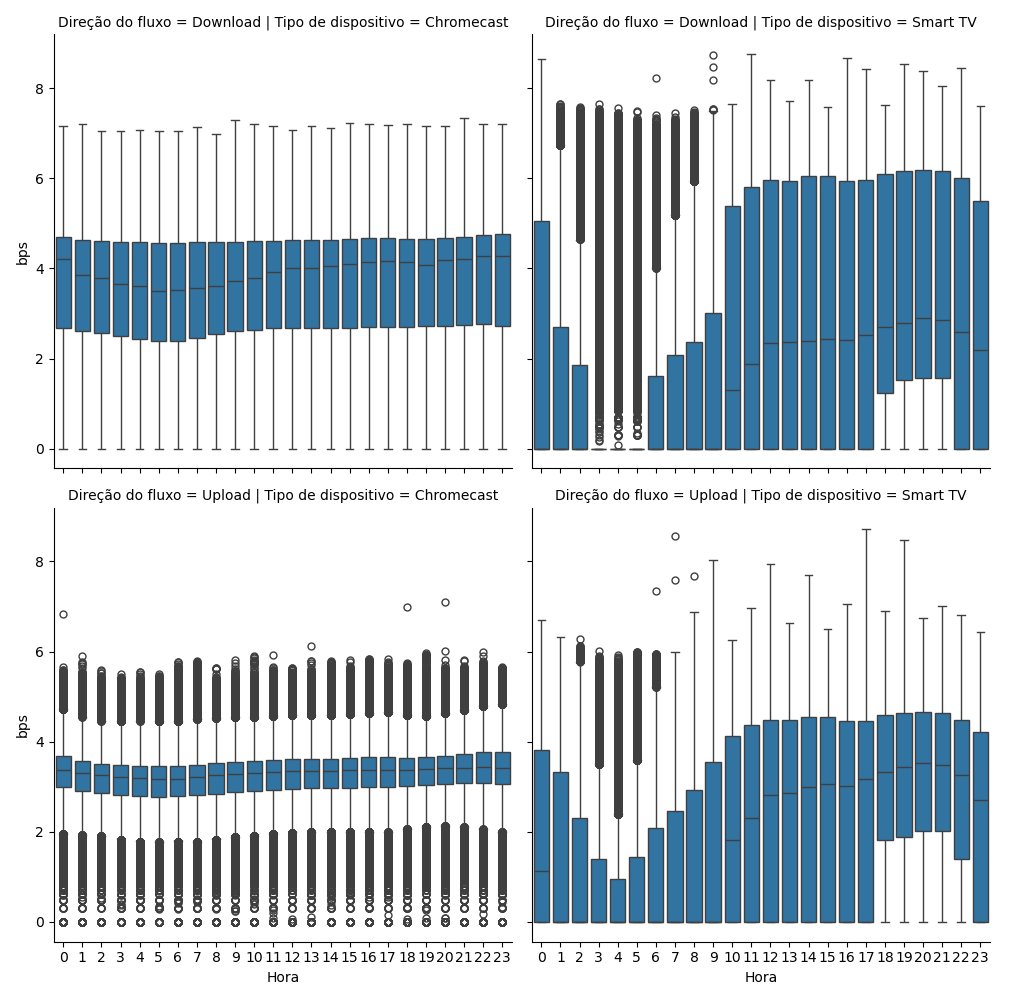
\includegraphics[width=\textwidth]{./resultados/questao3czero/boxplots.png}
	\label{fig:questao3-boxplots}
\end{figure}

Finalmente, os boxplots da figura~\ref{fig:questao3-boxplots} comparam as distribuições para diferentes horas do dia. Vemos que o chromecast possui um comportamento similar e estável ao longo do dia, seguindo o mesmo formato que os boxplots analisados na seção~\ref{sec:estatistica-geral}. Já para a Smart TV, vemos o impacto dos zeros afetando drasticamente o resultado dos boxplots ao longo do dia. As mesmas regiões descritas anteirormente se destacam nessa imagem, e nesse gráfico vemos que o vale contém basicamente todos os dados em um valor muito próximo de zero, com apenas outliers que chegam a taxas próximas às observadas nos horários comuns e de pico.

Nessa seção, podemos observar as seguintes características dos dados:
\begin{itemize}
	\item A presença de zeros no dataset impacta consideravelmente a maior e menor médias observadas, o que facilita a observação dos diferentes períodos de uso dos dispositivos.
	\item A Smart TV apresenta uma variação de uso ao longo do dia bem maior que o Chromecast, que é bem mais estável. Não é possível explicar o porquê desse comportamento.
	\item Através da Smart TV, é possível observar três padrões de comportamento distintos ao longo do dia, que são condizentes com o uso de televisão por uma população.
	\item A variância apresenta um decréscimo tanto no momento de menor uso quanto no momento de maior uso na Smart TV. Isso pode ser um resultado de mais dispositivos tendendo para um mesmo estado ``em uso'' ou ``desligado'' na qual a taxa consumida é constante e similar nesses dois cenários.
\end{itemize}

Por último, com base nos resultados da tabela~\ref{tab:questao3-estatisticas-horario}, pode-se encontrar os horários de maior média para serem utilizados na próxima seção. Esses horários estão representados na tabela~\ref{tab:questao3-horarios-picos}.

\begin{table}[h]
	\centering
	\begin{tabular}{lllr}
\toprule
 &  &  & 0 \\
Tipo de dispositivo & Direção do fluxo &  &  \\
\midrule
\multirow[t]{2}{*}{Chromecast} & Download & Média & 23 \\
\cline{2-4}
 & Upload & Média & 22 \\
\cline{1-4} \cline{2-4}
\multirow[t]{2}{*}{Smart TV} & Download & Média & 20 \\
\cline{2-4}
 & Upload & Média & 20 \\
\cline{1-4} \cline{2-4}
\bottomrule
\end{tabular}

	\caption{Horários de pico para cada dataset}
	\label{tab:questao3-horarios-picos}
\end{table}

\section{Análise dos horários de pico}
\label{sec:analise-pico}

Nessa seção, quer-se avaliar o comportamento dos dados nos horários de pico. Para isso, utilizamos a informação da tabela~\ref{tab:questao3-horarios-picos} para dividir os dados em quatro datasets distintos. Nesse caso, a tabela de dataset original é filtrada para conter apenas as entradas cujo horário na coluna ``Data e hora'' é o mesmo do que foi encontrado na seção anterior, para os quatro conjuntos de dados.

Nesse caso, o objetivo é caracterizar o comportamento dos dispositivos que estão transmitindo dados. Assim, não faz parte da análise predizer se um dispositivo vai transmitir ou não. Com isso, essa seção vai analisar os resultados para o dataset excluindo os valores nulos. Para fins de comparação, o histograma com a inclusão dos zeros também será apresentado.

\subsection{Metodologia}

A análise dessa seção consiste em fazer a estimação por máxima verossimilhança dos parâmetros das distribuições normal e gamma em cada um dos datasets. A estimação por MLE é desenvolvida no apêncide desse relatório, e nela é possível ver que não há uma forma fechada para a estimação dos parâmetros da função gamma. Portanto, essa estimação é feita utilizando soluções numéricas providenciadas pela biblioteca \texttt{scipy}. Uma vez que os parâmetros são encontrados, eles são utilizados para desenhar as curvas das PDFs teóricas juntos aos histogramas.

Após essa análise inicial, é feito o \textit{Probability plot} de cada um dos datasets, comparando-os com as distribuições normal e gamma. Finalmente, um QQPlot é feito para comparar os datasets do Chromecast e da Smart TV e identificar se o Download ou o upload é similar entre dispositivos.

\subsection{resultados}

As tabelas com os parâmetros encontrados são as tabelas~\ref{tab:questao4-mle-normal} e~\ref{tab:questao4-mle-gamma}, para a normal e a gamma respectivamente. O histograma que compara as PDFs pode ser visto na figura~\ref{fig:histogramas-ajuste}. O \textit{Probability Plot} para a normal e a gamma podem ser vistos nas figuras~\ref{fig:ppplot-normal} e~\ref{fig:ppplot-gamma}. Finalmente, a comparação entre os datasets através do QQPlot pode ser vista na figura~\ref{fig:qqplot}.

\begin{table}[h]
	\centering
	\begin{tabular}{llrr}
\toprule
 &  & mu & sigma2 \\
device_type & flow_type &  &  \\
\midrule
\multirow[t]{2}{*}{Chromecast} & bytes_down & 4.077841 & 1.438828 \\
 & bytes_up & 3.539628 & 0.731279 \\
\cline{1-4}
\multirow[t]{2}{*}{Smart TV} & bytes_down & 4.286281 & 2.002812 \\
 & bytes_up & 3.780892 & 1.162781 \\
\cline{1-4}
\bottomrule
\end{tabular}

	\caption{Estimação de parâmetros via MLE para a distribuição normal}
	\label{tab:questao4-mle-normal}
\end{table}

\begin{table}[h]
	\centering
	\begin{tabular}{llrr}
\toprule
 &  & $\alpha$ & $\lambda$ \\
Tipo de dispositivo & Direção do fluxo &  &  \\
\midrule
\multirow[t]{2}{*}{Chromecast} & Download & 7.870926 & 1.930165 \\
 & Upload & 23.287792 & 6.579145 \\
\cline{1-4}
\multirow[t]{2}{*}{Smart TV} & Download & 3.947653 & 0.920995 \\
 & Upload & 8.547361 & 2.260667 \\
\cline{1-4}
\bottomrule
\end{tabular}

	\caption{Estimação de parâmetros via MLE para a distribuição gamma}
	\label{tab:questao4-mle-gamma}
\end{table}

\begin{figure}[h]
	\centering
	\caption{Histogramas \textbf{com} a exclusão de entradas nulas. A curva azul é a normal e a curva laranja é a gamma.}
	\includegraphics[width=\textwidth]{./resultados/questao4/histogramas.png}
	\label{fig:histogramas-ajuste}
\end{figure}

Na figura~\ref{fig:histogramas-ajuste}, podemos comparar os histogramas as distribuições cujos parâmetros foram estimados pela estimação de máxima verossimilhança. Esses parâmetros estão descritos nas tabelas~\ref{tab:questao4-mle-normal} e~\ref{tab:questao4-mle-gamma}. Vemos que ambos os ajustes feitos seguem razoavelmente bem os histogramas. As piores representações ficam para os histogramas multimodais observados para os dados de Download de ambos os dispositivos.

A figura~\ref{fig:histogramas-ajuste-czero} mostra qual seria o resultado dos ajustes caso os zeros não fossem desconsiderados. Temos que o caso do Chromecast é pouco alterado, com a distribuição gamma apresentando um \textit{skew} maior para a esquerda, em direção aos valores nulos. Já o dataset da Smart TV é amplamente prejudicado, com a distribuição normal obtendo valores de $\sigma^2$ maiores do que o caso anterior e a distribuição gamma se concentrando completamente nos valores nulos. Vemos que as distribuições nesse caso seriam uma péssima representação dos dados observados. Isso se dá porque esses datasets refletem a união de dois comportamentos distintos: Dispositivos desligados (taxa nula) e dispositivos ligados (taxa não nula). Uma distribuição ajustada nesse dataset não seria capaz de representar esse comportamento de estados internos.

\begin{figure}[h]
	\centering
	\caption{Histogramas \textbf{sem} a exclusão de entradas nulas. A curva azul é a normal e a curva laranja é a gamma.}
	\includegraphics[width=\textwidth]{./resultados/questao4czero/histogramas.png}
	\label{fig:histogramas-ajuste-czero}
\end{figure}


\begin{figure}[h]
	\centering
	\caption{\textit{Probability Plot} para a distribuição normal}
	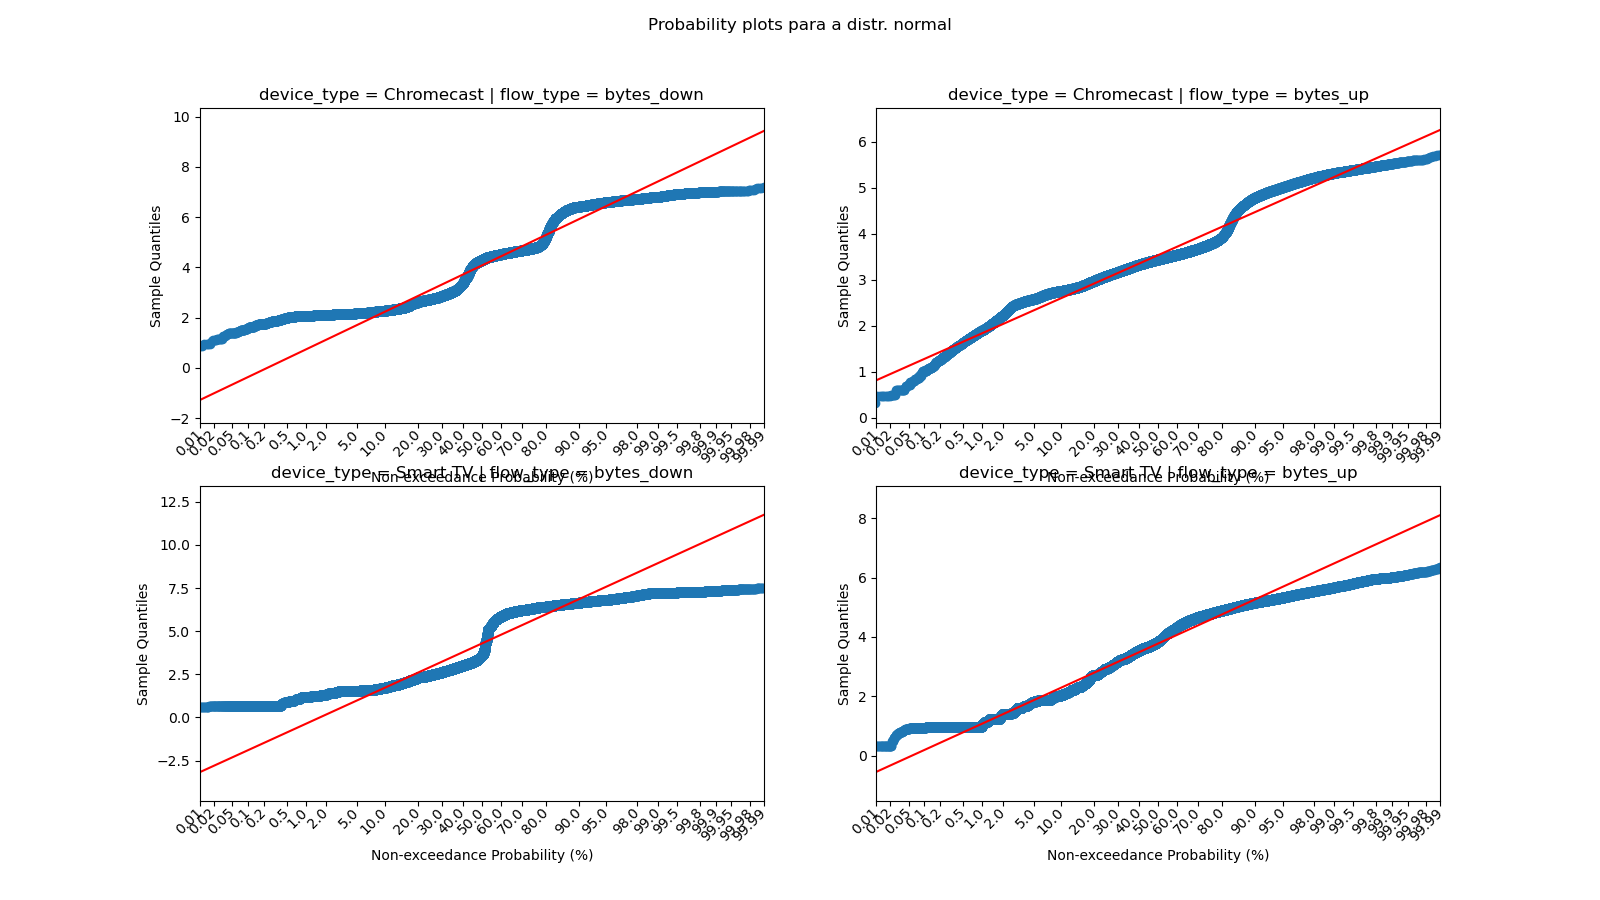
\includegraphics[width=\textwidth]{./resultados/questao4/probability_plots_normal.png}
	\label{fig:ppplot-normal}
\end{figure}

\begin{figure}[h]
	\centering
	\caption{\textit{Probability Plot} para a distribuição gamma}
	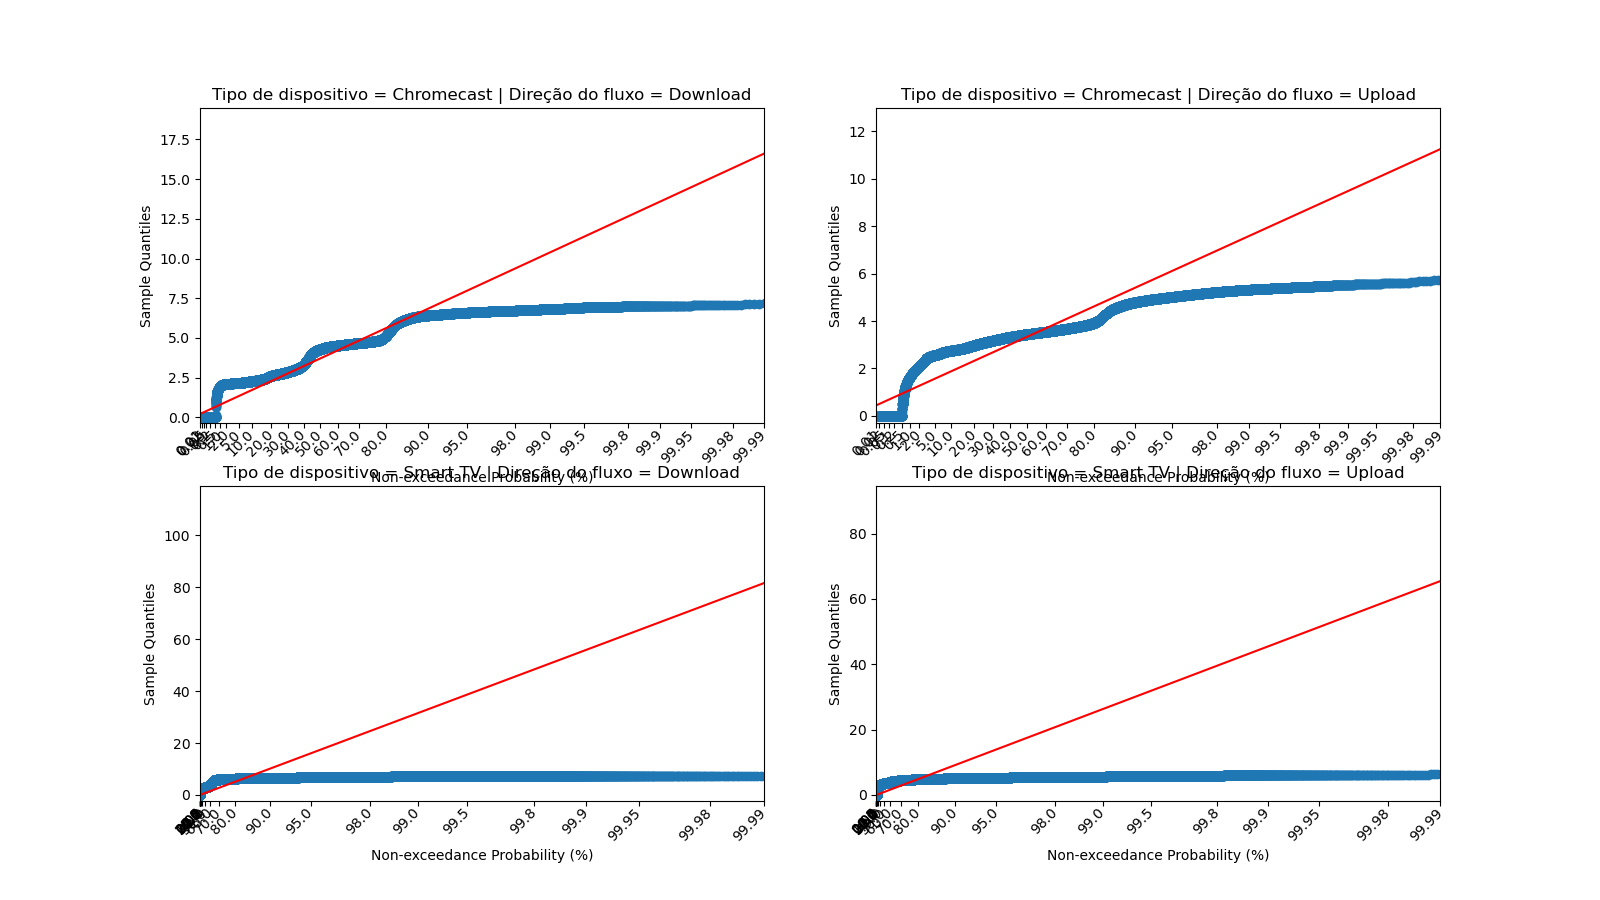
\includegraphics[width=\textwidth]{./resultados/questao4/probability_plots_gamma.png}
	\label{fig:ppplot-gamma}
\end{figure}

Os \textit{Probability plots} das figuras~\ref{fig:ppplot-normal} e~\ref{fig:ppplot-gamma} mostram o quão bem os datasets seguem as distribuições normal e gamma, respectivamente. De todos os 8 gráficos, o gráfico que mais se aproxima visualmente da linha de 45$\degree$ é a curva de upload do Chromecast para a distribuição normal. Esse resultado pode ser comparado com o histograma: A região entre o percentil 80\% e 95\% da distribuição, a curva em formato de ``S'' observada no gráfico bate com a ``menor coluna do meio'', a coluna do 4 $\log(\text{bps})$, no histograma. Exceto também pela coluna mais alta, quase todas as colunas do histograma ficam próximas à curva da normal. Portanto, isso indica que o Upload do Chromecast pode ser substituído por uma variável aleatória normal com os parâmetros iguais aos da tabela~\ref{tab:questao4-mle-normal}.

\begin{figure}[h]
	\centering
	\caption{QQPlots}
	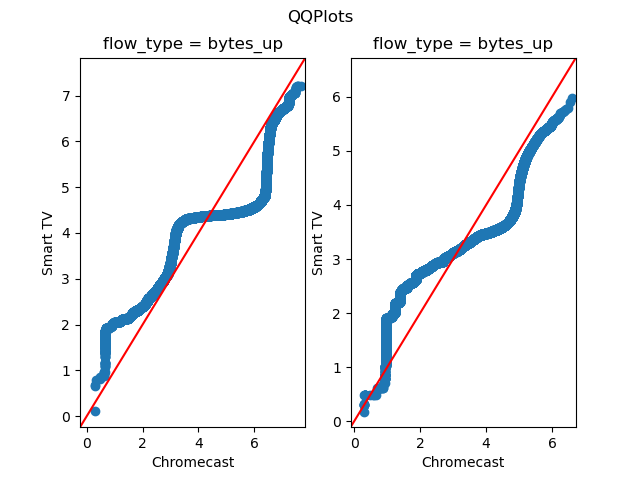
\includegraphics[width=\textwidth]{./resultados/questao4/qqplots.png}
	\label{fig:qqplot}
\end{figure}

O QQPlot da figura~\ref{fig:qqplot} tenta determinar se o fluxo de download e upload entre os dispositivos segue a mesma distribuição. Nenhum dos gráficos é suficientemente próximo a curva de 45$\degree$, mas é possível observar que os datasets de upload tem uma similaridade maior do que os datasets de upload.

Portanto, as principais conclusões dessa seção são:
\begin{itemize}
	\item Os horários de pico escolhidos estão na tabela~\ref{tab:questao3-horarios-picos}
	\item A exclusão dos zeros é necessária nessa seção, já que se quer avaliar a distribuição resultante dos dispositivos que estão transmitindo dados. A não exclusão dos zeros resulta em um ajuste ruim de curvas.
	\item Os melhores ajustes de curva com base nos histogramas estão para os dados de Upload, já que os dados de download apresentam um comportamento multimodal.
	\item A melhor curva de \textit{Probability Plot} é para o upload do Chromecast, e dado que a curva mantém-se na mesma direção ao longo de todo o gráfico, pode-se caracterizar esse dataset como uma variável aleatória normal.
	\item Com base no QQPlot, não é possível dizer que os datasets do Chromecast é similar ao da Smart TV, para nenhum dos dois casos.
\end{itemize}


\section{Análise de correlação}

Nessa seção, será feita uma análise de correlação entre as taxas de download e upload dos dispositivos. Nesse caso, a estrututra do dataset é diferente da utilizada até então: Ao invés da coluna categórica ``Direção do fluxo'' para dizer se o valor é de upload ou de download, há duas colunas: Uma para o valor da taxa de upload e outro para a taxa de download.

Nesse caso, é desejado avaliar a correlação incluindo todos os dados. Se a hipótese de que alguns dispositivos possuem taxa nula porque estão desligados, essas taxas devem ser nulas tanto para upload quanto para download, o que não vai prejudicar o resultado da correlação tanto quanto uma variável livre e outra nula fariam. Porém, múltiplas entradas do vetor $(0,0)$ podem introduzir um viés que incrementa artificialmente o resultado de correlação de pearson. Portanto, para avaliar a estatística, ambas as alternativas (com e sem os zeros) serão avaliadas.

Nessa seção, decidiu-se por avaliar a correlação entre taxas de download e upload que ocorrem na mesma hora, já que não é possível associar taxas de upload e download que aconteceram em horários diferentes. Assim, já que o upload e o download do Chromecast acontecem em horários distintos, decidiu-se por avaliar a correlação em \textbf{três} datasets diferentes:
\begin{itemize}
	\item Chromecast as 23hrs
	\item Chromecast as 22hrs
	\item Smart TV as 20hrs
\end{itemize}

\subsection{Metodologia}

Para remover os zeros do dataset, o dataset é filtrado de modo que, se pelo menos uma entrada de bps (download ou upload) é zero, toda a entrada é removida. Isso vai remover tanto os pontos $(0,0)$ repetidos como qualquer ponto $(0,x)$ e $(0,y)$.

A correlação de pearson é calculada utilizando a biblioteca \texttt{scipy}, que retorna a estatística e o valor-p associado.

\subsection{Resultados}

Os resultados das estatísticas podem ser vistos nas tabelas~\ref{tab:questao5-resultados-correlacao} e~\ref{tab:questao5-resultados-correlacao-semzero}, para resultados com valores nulos e sem valores nulos respectivamente. Já o scatter plot pode ser visto na figura~\ref{fig:questao5-scatter-plots}.

Podemos ver através das tabelas~\ref{tab:questao5-resultados-correlacao} e~\ref{tab:questao5-resultados-correlacao-semzero} que a presença ou não das entradas nulas pouco influenciou no resultado da correlação, que indica uma correlação forte ($\rho>0.7$) em todos os casos, com um valor-p menor que 7 casas decimais. O resultado positivo de todos os casos indica que o valor de upload tende a crescer quando o valor de download cresce, e vice-versa. Porém, esse resultado não nos dá mais informações a respeito do tipo de relação e nem a taxa de crescimento de uma variável em função da outra.

Com base no gráfico da figura~\ref{fig:questao5-scatter-plots}, podemos observar que os dados apresentam uma correlação positiva com o tipo de correlação difícil de distinguir devido a quantidade excessiva de pontos. Pode-se dizer que o segundo e o terceiro gráfico aparentam possuir correlações lineares, mas o primeiro apresenta uma tendência de seguir um ``S'', que claramente é não linear. Vemos que o impacto das entradas nulas é observado devido aos dois conjunto de pontos que se apresentam em $(x,0)$ e $(0,y)$, muito mais predominantes no caso do Smart TV do que no caso do Chromecast.

\begin{table}[h]
	\centering
	\begin{tabular}{llrr}
\toprule
 &  & rho & p-value \\
hour & device_type &  &  \\
\midrule
20 & Smart TV & 0.900466 & 0.000000 \\
\cline{1-4}
22 & Chromecast & 0.776669 & 0.000000 \\
\cline{1-4}
23 & Chromecast & 0.792728 & 0.000000 \\
\cline{1-4}
\bottomrule
\end{tabular}

	\caption{Resultados da correlação de pearson sem exclusão de zeros}
	\label{tab:questao5-resultados-correlacao}
\end{table}

\begin{table}[h]
	\centering
	\begin{tabular}{llrr}
\toprule
 &  & rho & p-value \\
hour & device_type &  &  \\
\midrule
20 & Smart TV & 0.900466 & 0.000000 \\
\cline{1-4}
22 & Chromecast & 0.776669 & 0.000000 \\
\cline{1-4}
23 & Chromecast & 0.792728 & 0.000000 \\
\cline{1-4}
\bottomrule
\end{tabular}

	\caption{Resultados da correlação de pearson com exclusão de zeros}
	\label{tab:questao5-resultados-correlacao-semzero}
\end{table}

\begin{figure}[h]
	\centering
	\caption{Gráficos de correlação entre os datasets sem exclusão de zeros}
	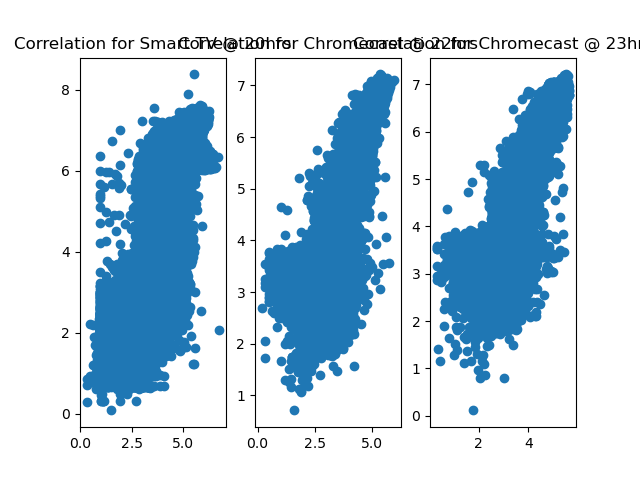
\includegraphics[width=\textwidth]{./resultados/questao5czero/correlation_plots.png}
	\label{fig:questao5-scatter-plots}
\end{figure}

Com isso, pudemos concluir nessa seção que
\begin{itemize}
	\item Três datasets com horários de pico distintos devem ser analizados para fazer uma correlação justa (upload e download no mesmo horário).
	\item As taxas de upload e download possuem uma forte correlação positiva entre si durante horários de pico, independente se o dataset contém as entradas nulas ou não.
	\item Os gráficos scatter sugerem uma relação linear entre as entradas do Chromecast, mas uma relação não-linear (formato de ``s'') no caso da Smart TV.
\end{itemize}

\section{G-Test}

O G-Test é um teste de hipótese que avalia se dois datasets, com lista de frequências de observação, possuem distribuições similares. Nessa seção, queremos observar se as distribuições para as taxas de upload e download são similares entre um mesmo dispositivo nos horários de pico. Para isso, serão comparados os mesmos datasets da seção anterior.

\subsection{metodologia}

Para o cálculo do G-Test, é necessário criar duas listas de frequências, uma para cada distribuição, e compará-las no teste. Essa lista de frequências é equivalente ao resultado numérico de um histograma, onde cada bin representa o intervalo e a contagem é a frequência de observações desse intervalo. Com isso, utilizou-se funções da biblioteca \texttt{numpy} para encontrar os intervalos dos bins apropriados segundo a regra de sturges para as taxas de download. Após isso, os mesmos intervalos dos bins são utilizados para fazer a contagem da taxa de upload e da taxa de download, e ambas as contagens são passadas para a função que calcula a estatística.

\subsection{resultados}

Os resultados da estatística e do valor-p podem ser vistos na tabela~\ref{tab:g-test}.

\begin{table}[h]
	\centering
	\begin{tabular}{llrr}
\toprule
 &  & statistic & p-value \\
hour & device_type &  &  \\
\midrule
20 & Smart TV & 464123.754381 & 0.000000 \\
\cline{1-4}
22 & Chromecast & 147134.065797 & 0.000000 \\
\cline{1-4}
23 & Chromecast & 139680.940307 & 0.000000 \\
\cline{1-4}
\bottomrule
\end{tabular}

	\caption{Resultados G-Test}
	\label{tab:g-test}
\end{table}

Como podemos ver, os resultados são bem diferentes entre si, e o valor-p é menor que 7 casas decimais. Portanto, todas as hipóteses que as distribuições são iguais foram rejeitadas. Esse resultado era esperado dado as observações das seções anteriores: Os histogramas entre as taxas de download e upload possuem formatos diferentes, onde uma é multimodal e a outra não.

Com isso, nessa seção podemos simplesmente concluir que todos os testes de hipótese foram rejeitados, ou seja, nenhuma distribuição de upload é similar a de download.

\section{Considerações finais}

Nesse trabalho, foram observados os dados de taxa de upload e download de dois tipos de dispositivos: Smart TVs e Chromecasts, que foram coletados por uma ISP de médio porte.

Através desses dados, foi possível observar diferenças no comportamento de upload e de download dos dispositivos, que resultam em distribuições diferentes; observar padrões de uso desses dispositivos que variam em função da hora do dia, observar correlações entre taxas e comparar o comportamento desse dataset com o comportamento de distribuições teóricas.

A análise sobre a exclusão ou não dos valores nulos trouxe uma discussão a respeito da interpretação dos dados e dos diferentes casos onde essa informação é relevante ou não é relevante. Algumas comparações foram feitas entre os datasets com e sem a presença de valores nulos e foi possível observar o impacto dessas amostras nos resultados. A presença ou não dos zeros só será definida ao definir um objetivo específico para a análise.

\end{document}

